\documentclass[preview]{standalone}

\usepackage{amsmath}
\usepackage{amssymb}
\usepackage{stellar}
\usepackage{definitions}
\usepackage{gensymb}
\usepackage{tikz}

\newcommand{\cel}{C\degree}

\begin{document}

\id{fisica-termodinamica}
\genpage

\section{Termodinamica}

\begin{snippet}{termodinamica-expl1}
    La \textbf{temperatura} è una grandezza operativa (\cel, K)
    mentre il \textbf{calore} è una forma di energia (Joule).
    
    Tipi di termometro: \textit{dilatazione} (es. mercurio),
    \textit{contatto} (tensione in funzione della temperatura),
    \textit{infrarossi} (potenza onda infrarossi riflessa).
    
    La pressione di vari gas confinati è linearmente proporzionale alla temperatura.
    Tutte le funzioni lineari della pressione \(P(T)\) hanno lo stesso punto in comune;
    quando la temperatura è \(0\) (zero assoluto).
\end{snippet}

\section{Dilatazione}

\subsection{Solidi}

\begin{snippetdefinition}{dilatazione-solido-definition}{Dilatazione solido}
    La dilatazione di un oggetto in una direzione \(\Delta l\) in funzione del
    cambio di temperatura \(\Delta T\) è proporzionale e data da
    \[
        \Delta l = l_0 \cdot \alpha \cdot \Delta T
    \]
    dove \(l_0\) è la lunghezza iniziale e \(\alpha\) è il coefficiente di dilatazione lineare
    \((\frac{1}{K})\). Questo funziona solamente per certi intervalli di temperatura,
    ossia il solido non deve cambiare stato.
    
    Un solido si dilata in tutte le direzioni.
    La dilatazione dell'area o del volume di un solito possono essere \textit{approssimate}
    nella seguente maniera
    \begin{align*}
        \Delta A &\approx 2 \cdot A_0 \cdot \alpha \cdot \Delta T \\
        \Delta V &\approx 3 \cdot V_0 \cdot \alpha \cdot \Delta T
    \end{align*}
\end{snippetdefinition}

\subsection{Fluidi (liquidi e gas)}

\begin{snippetdefinition}{dilatazione-volumetrica-definition}{Dilatazione volumetrica}
    Un liquido/gas, non avendo forma propria, ha una dilatazione che può essere
    quantificata solo in termini volumetrici
    \[
        \Delta V = V_0 \cdot \gamma \cdot \Delta T
    \]
    dove \(\gamma\) è il coefficiente di dilatazione cubica.
\end{snippetdefinition}

\section{Gas}

\subsection{Trasformazione isobarica}

\begin{snippet}{trasformazione-isobarica-illustration}
    \begin{minipage}[left]{0.25\textwidth}
        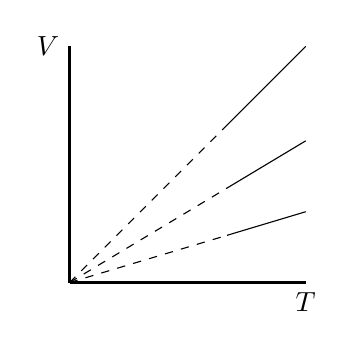
\begin{tikzpicture}
            \draw[-, thick] (0,0) -- (3,0) node[below] {\(T\)};
            \draw[-, thick] (0,0) -- (0,3) node[left] {\(V\)};
    
            \draw[-, dashed] (0,0) -- (2,0.6);
            \draw[-] (2,0.6) -- (3,0.9);
    
            \draw[-, dashed] (0,0) -- (2,2);
            \draw[-] (2,2) -- (3,3);
    
            \draw[-, dashed] (0,0) -- (2,1.2);
            \draw[-] (2,1.2) -- (3,1.8);
        \end{tikzpicture}
    \end{minipage}
    \begin{minipage}[left]{0.75\textwidth}
    Cambiamento dello stato quando la pressione è costante.
    \[
        \frac{V_1}{T_1} = \frac{V_2}{T_2}
    \]
    \end{minipage}
\end{snippet}

\subsection{Trasformazione isocòra}

\begin{snippet}{trasformazione-isocora-illustration}
    \begin{minipage}[left]{0.25\textwidth}
        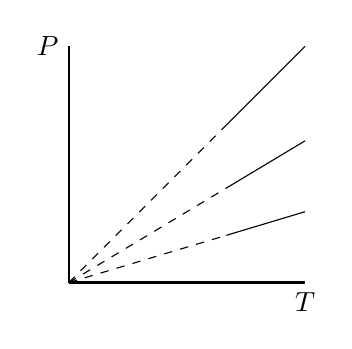
\begin{tikzpicture}
            \draw[-, thick] (0,0) -- (3,0) node[below] {\(T\)};
            \draw[-, thick] (0,0) -- (0,3) node[left] {\(P\)};

            \draw[-, dashed] (0,0) -- (2,0.6);
            \draw[-] (2,0.6) -- (3,0.9);

            \draw[-, dashed] (0,0) -- (2,2);
            \draw[-] (2,2) -- (3,3);

            \draw[-, dashed] (0,0) -- (2,1.2);
            \draw[-] (2,1.2) -- (3,1.8);
        \end{tikzpicture}
    \end{minipage}
    \begin{minipage}[left]{0.75\textwidth}
    Cambiamento dello stato quando il volume rimane costante.
    \[
        \frac{P_1}{T_1} = \frac{P_2}{T_2}
    \]
    \end{minipage}
\end{snippet}

\subsection{Trasformazione isotermica}

\begin{snippet}{trasformazione-isotermica-illustration}
    \begin{minipage}[left]{0.25\textwidth}
        \begin{tikzpicture}
            \draw[-, thick] (0,0) -- (3,0) node[below] {\(V\)};
            \draw[-, thick] (0,0) -- (0,3) node[left] {\(P\)};

            \draw[domain=0.5:2.25, smooth, variable=\x]  plot ({1 / \x}, {\x});
        \end{tikzpicture}
    \end{minipage}
    \begin{minipage}[left]{0.75\textwidth}
    Cambiamento dello stato quando la temperatura è costante.
    \[
        P_1 \cdot V_1 = P_2 \cdot V_2
    \]
    \end{minipage}
\end{snippet}

\subsection{Gas perfetti}

\begin{snippetdefinition}{gas-perfetto-definition}{Gas perfetto}
    Un gas \textit{perfetto} rispetta tutte e 3 le leggi assieme
\[
    \frac{P_1 \cdot V_1}{T_1} = \frac{P_2 \cdot V_2}{T_2}
\]
\end{snippetdefinition}

\subsubsection{Equazione di stato dei gas perfetti}

\begin{snippet}{equazione-fas-perfetti}
    Un gas perfetto rispetta l'identità
    \[
        pV = nRT
    \]
    dove
    \begin{itemize}
        \item \(p\): Pressione
        \item \(V\): Volume
        \item \(n\): Numero di moli
        \item \(R\): Costante universale dei gas \(8.314 \frac{J}{\text{mol} \cdot K}\)
        \item \(T\): Temperatura
    \end{itemize}
\end{snippet}

\section{Calore}

\subsection{Capacità termica}

\begin{snippetdefinition}{capacita-termica-definition}{Capacità termica}
    La capacità termica di un sistema è la capacità di
    cambiare temperatura scambiando calore (energia).
    \[
        C=\frac{Q}{\Delta T}, \quad \left[\frac{\text{J}}{\text{K}}\right]
    \]
    dove \(C\) è la capacità termica.
    \(Q\) è il calore scambiato e \(\Delta T\) è la variazione di temperatura.

    La capacità termica di un sistema con più sostanze è data dalla somma
    delle singole capacità termiche.
    \[
        C_{\text{system}} = \sum_j C_j
    \]
\end{snippetdefinition}

\subsection{Calore specifico}

\begin{snippetdefinition}{calore-specifico-definition}{Calore specifico}
    Il calore specifico determina la capacità termica per unità di massa.
    Corrisponde alla quantità di calore (energia) necessaria per innalzare,
    o diminuire, di un unità la temperatura di una quantità di sostanza.
    \[
        c_s = \frac{C}{m}, \quad \left[\frac{\text{J}}{\text{K}\cdot \text{Kg}}\right]
    \]
    dove \(c_s\) è il calore specifico. \(C\) è la capacità termica
    e \(m\) è la massa.
\end{snippetdefinition}

\subsection{Calore latente}

\begin{snippetdefinition}{calore-latente-definition}{Calore latente}
    Il calore latente è la quantità di energia per massa
    durante lo svolgimento di un passaggio di stato.
    \[
        L=\frac{Q}{m}, \quad \left[\frac{\text{J}}{\text{Kg}}\right]
    \]
\end{snippetdefinition}

\section{Coefficienti di dilatazione}

\begin{snippet}{coefficienti-dilatazione}
    \begin{center}
        \begin{tabular}{ l | c | c }
            \hline
            \textbf{Sostanza} & \textbf{Coeff lineare \(\alpha\,[K^{-1}]\)} & \textbf{Coeff volumetrica \(\gamma\,[K^{-1}]\)} \\
            \hline
            Alluminio & \(23 \cdot 10^{-6}\) & \(69 \cdot 10^{-6}\) \\
            Ottone & \(19 \cdot 10^{-6}\) & \(57 \cdot 10^{-6}\) \\
            Calcestruzzo & \(12 \cdot 10^{-6}\) & \(36 \cdot 10^{-6}\) \\
            Rame & \(17 \cdot 10^{-6}\) & \(51 \cdot 10^{-6}\) \\
            Vetro comune & 8.\(5 \cdot 10^{-6}\) & \(26 \cdot 10^{-6}\) \\
            Vetro Pirex & 3.\(3 \cdot 10^{-6}\) & 9.\(9 \cdot 10^{-6}\) \\
            Oro & \(14 \cdot 10^{-6}\) & \(42 \cdot 10^{-6}\) \\
            Ferro o Acciaio & \(12 \cdot 10^{-6}\) & \(36 \cdot 10^{-6}\) \\
            Piombo & \(29 \cdot 10^{-6}\) & \(87 \cdot 10^{-6}\) \\
            Argento & \(19 \cdot 10^{-6}\) & \(57 \cdot 10^{-6}\) \\
            Benzene & - & \(1240 \cdot 10^{-6}\) \\
            Alcol etilico & - & \(1120 \cdot 10^{-6}\) \\
            Benzina & - & \(950 \cdot 10^{-6}\) \\
            Mercurio & - & \(182 \cdot 10^{-6}\) \\
            Alcol metilico & - & \(1200 \cdot 10^{-6}\) \\
            Acqua & - & \(207 \cdot 10^{-6}\) \\
            \hline  
        \end{tabular}
    \end{center}
    \phantom{}
\end{snippet}

\section{Unità di misura}

\begin{snippet}{unita-di-misura-lista}
    \begin{align*}
        \cel \to K&: \quad \cel+273.15 \\
        \text{in} \to \text{cm}&: \quad \text{in} \cdot 2.54 \\
        \text{F} \to \text{\cel}&: \quad (\text{F} - 32) \cdot \frac{5}{9} \\
        \text{mi} \to \text{m}&: \quad \text{mi} \cdot 1609 \\
        \text{ft} \to \text{m}&: \quad \text{ft} \cdot 0.3048 \\
        \text{yd} \to \text{m}&: \quad \text{yd} \cdot 0.9144 \\
        \text{HP} \to \text{CV}&: \quad \text{HP} \cdot 1.01 \\
    \end{align*}
    \phantom{}
\end{snippet}

\end{document}